\section{Experimental Analysis}\label{sec:experiments}
% summary

% benchmark algorithm
To benchmark the performance of MLEMTRL, we compare ourselves to a posterior sampling method (\textbf{PSRL})~\citep{osband2013more}, equipped with a combination of product-Dirichlet and product-Normal Inverse Gamma priors for the tabular setting, and Bayesian Multivariate Regression prior~\citep{minka2000bayesian} for the continuous setting. In PSRL, at every round, a new model is sampled from the prior, and it learns in the target MDP from scratch. Finally, for model-based planning, we use \textsc{RiccatiIterations} to obtain the optimal linear controller for the sampled model. In the continuous action setting, we compare the performance to the baseline algorithm multi-task soft-actor critic (\textbf{MT-SAC})~\citep{haarnoja2018soft, yu2020meta} and a modified \textbf{MT-SAC-TRL} using data from the novel task during learning. In the tabular MDP setting, we compare against multi-task proximal policy optimisation (\textbf{MT-PPO)}~\citep{schulman2017proximal, yu2020meta} and similarly \textbf{MT-PPO-TRL}.%\\ 



%The objectives of our empirical study are two-fold:
\textit{The objectives of our empirical study are three-fold:}%\vspace*{-.4em}
\begin{enumerate}
    \item How does \textsc{MLEMTRL} impact performance in terms of \textbf{learning speed}, \textbf{jumpstart improvement} and \textbf{asymptotic convergence} compared to our baseline?
    \item What is the performance loss of \textsc{MLEMTRL} in the \textbf{non-realisable setting}?
    \item How does Meta-MLEMTRL perform in the \textbf{non-realisable setting}?
\end{enumerate}

We conduct two kinds of experiments to verify our hypotheses. Firstly, in the upper row of Figure~\ref{fig:full_results}, we consider the realisable setting, where the novel task $\mu^*$ is part of the convex hull $\mathcal{C}(\mathcal{M}_s)$. In this case, we are looking to identify an improvement in some or all of the aforementioned qualities compared to the baselines.
Further, in the bottom row of Figure~\ref{fig:full_results}, we investigate whether the algorithm can generalise to the case beyond what is supported by the theory in Section~\ref{subsec:realisable}. We begin by recalling the goals of the transfer learning problem~\citep{langley2006transfer}.%\\


%We conduct two kinds of experiments to verify our hypotheses. Firstly, in Figure~\ref{fig:time}, we compare the performance of MLEMTRL to PSRL~\citep{osband2013more} in terms of learning speed and jumpstart improvement. We also identify a zero or near-zero regret for MDPs satisfying the realisability conditions in Section~\ref{subsec:realisable}. Lastly, we see a trend of increase in regret with an increase in \emph{Kullback-Leibler divergence} of the true MDP $\mdp^{*}$ from our estimate, $\hat{\mdp}$. In another experiment, in Figure~\ref{fig:norms}, we further verify the relation between increase in divergence and increase in regret. We begin by recalling the goals of the transfer learning problem~\citep{langley2006transfer}.

\noindent1. \textit{Learning Speed Improvement:}
A learning speed improvement would be indicated by the algorithm reaching its asymptotic convergence with less data.\\
\noindent2. \textit{Asymptotic Improvement:}
 An asymptotic improvement would mean the algorithm converges asymptotically to a superior solution to that one of the baseline.\\
\noindent3. \textit{Jumpstart Improvement:}
A jumpstart improvement can be verified by the behaviour of the algorithm during the early learning process. In particular, if the algorithm starts at a better solution than the baseline, or has a simpler optimisation surface, it may more rapidly approach better solutions with much less data.%\\
%\iffalse
%\begin{figure}[t!]
%    \centering
%    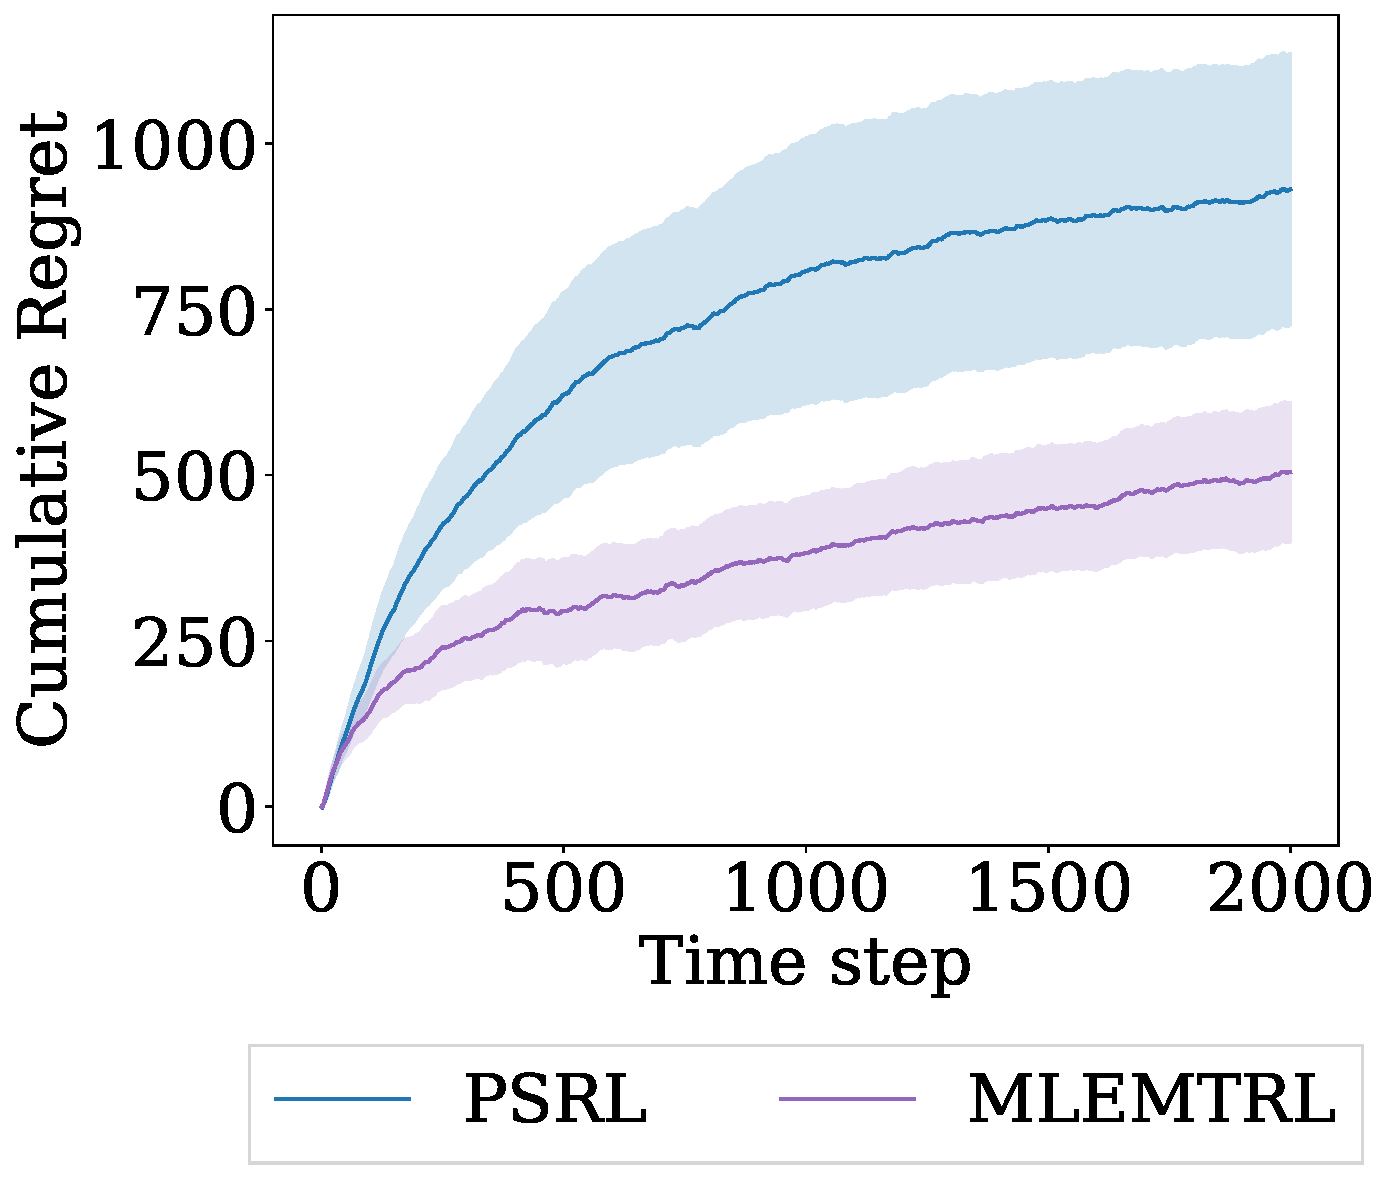
\includegraphics[width=0.4\textwidth]{img/chain_experiment.pdf}
%    \caption{This visualisation is of multiple variants of the Chain environment. Here, the slippage parameter is being varied. The cumulative regret is shown over the first $2000$ time steps and the shaded regions represent the $95\%$ confidence interval of the cumulative regret for the two algorithms. The agents update their policies every $20$ steps. For regret, lower values are better.}\label{fig:chain}\vspace*{-1em}
%\end{figure}
%\fi

\setlength{\textfloatsep}{4pt}%
\begin{figure}[t!]
    \centering
    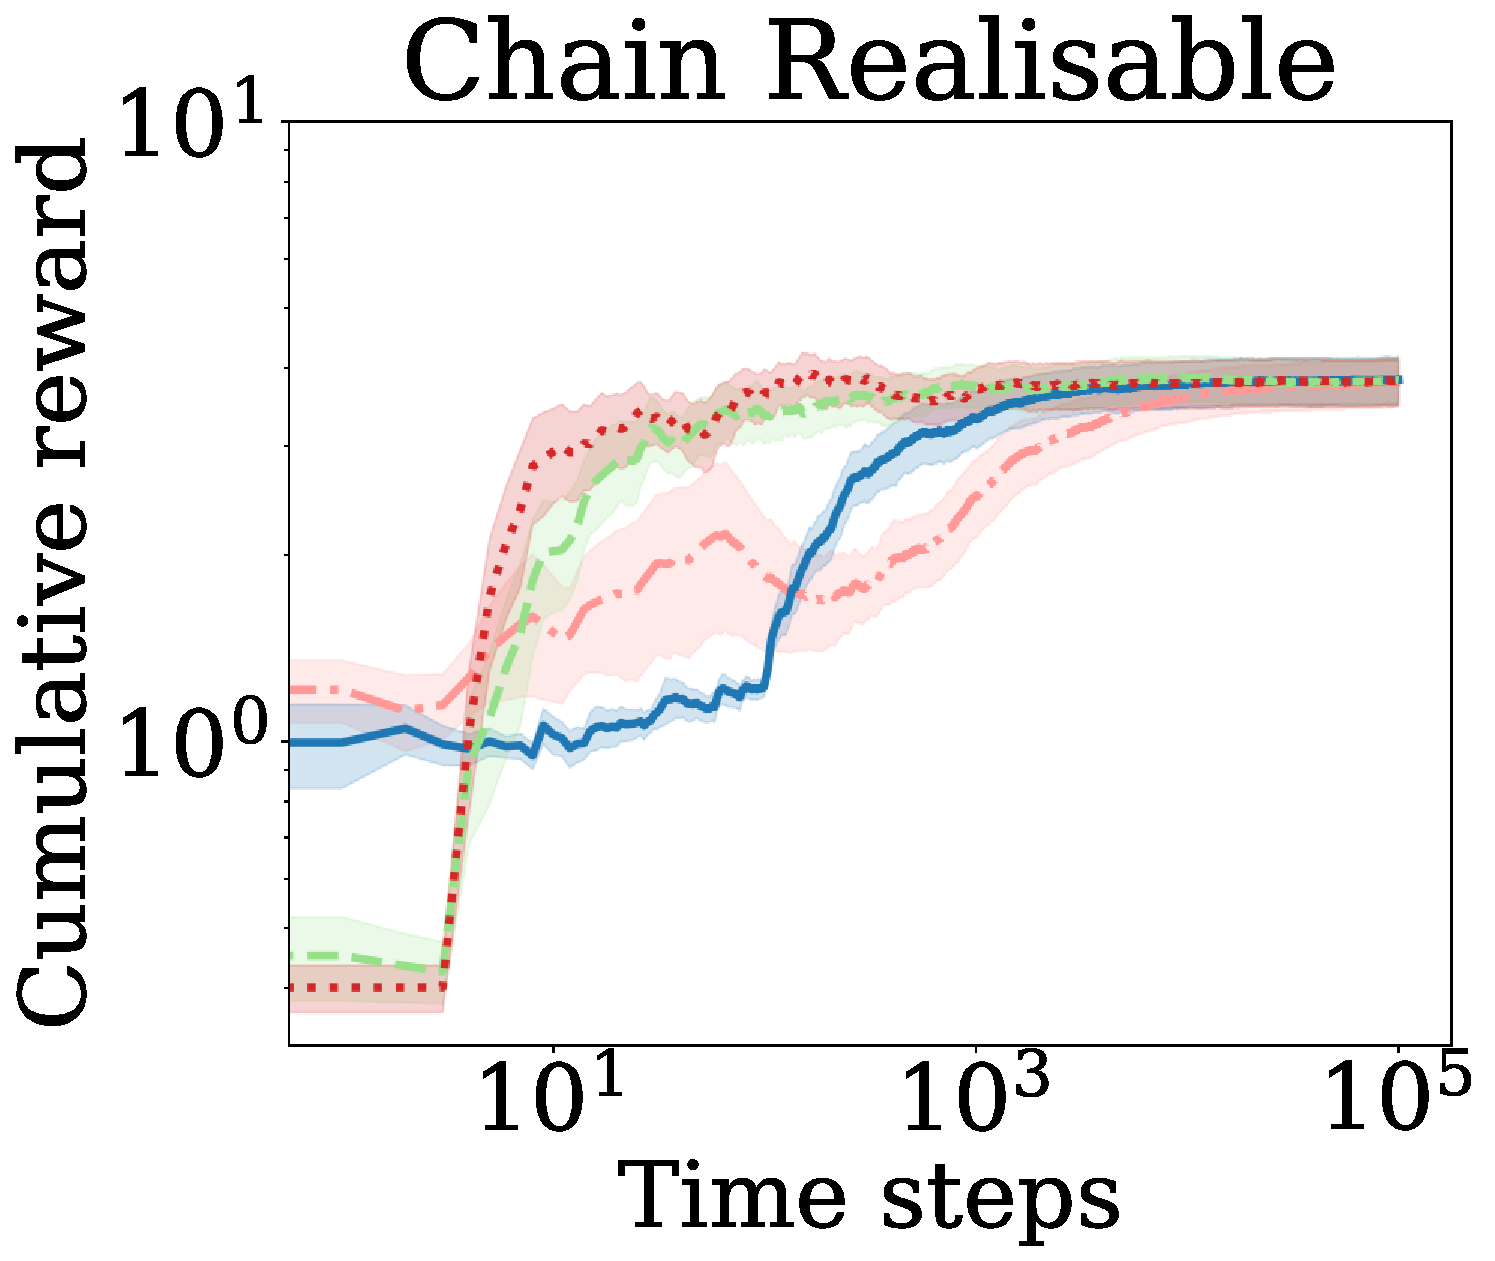
\includegraphics[width=0.3\textwidth]{img/chain_realisable.pdf}         
    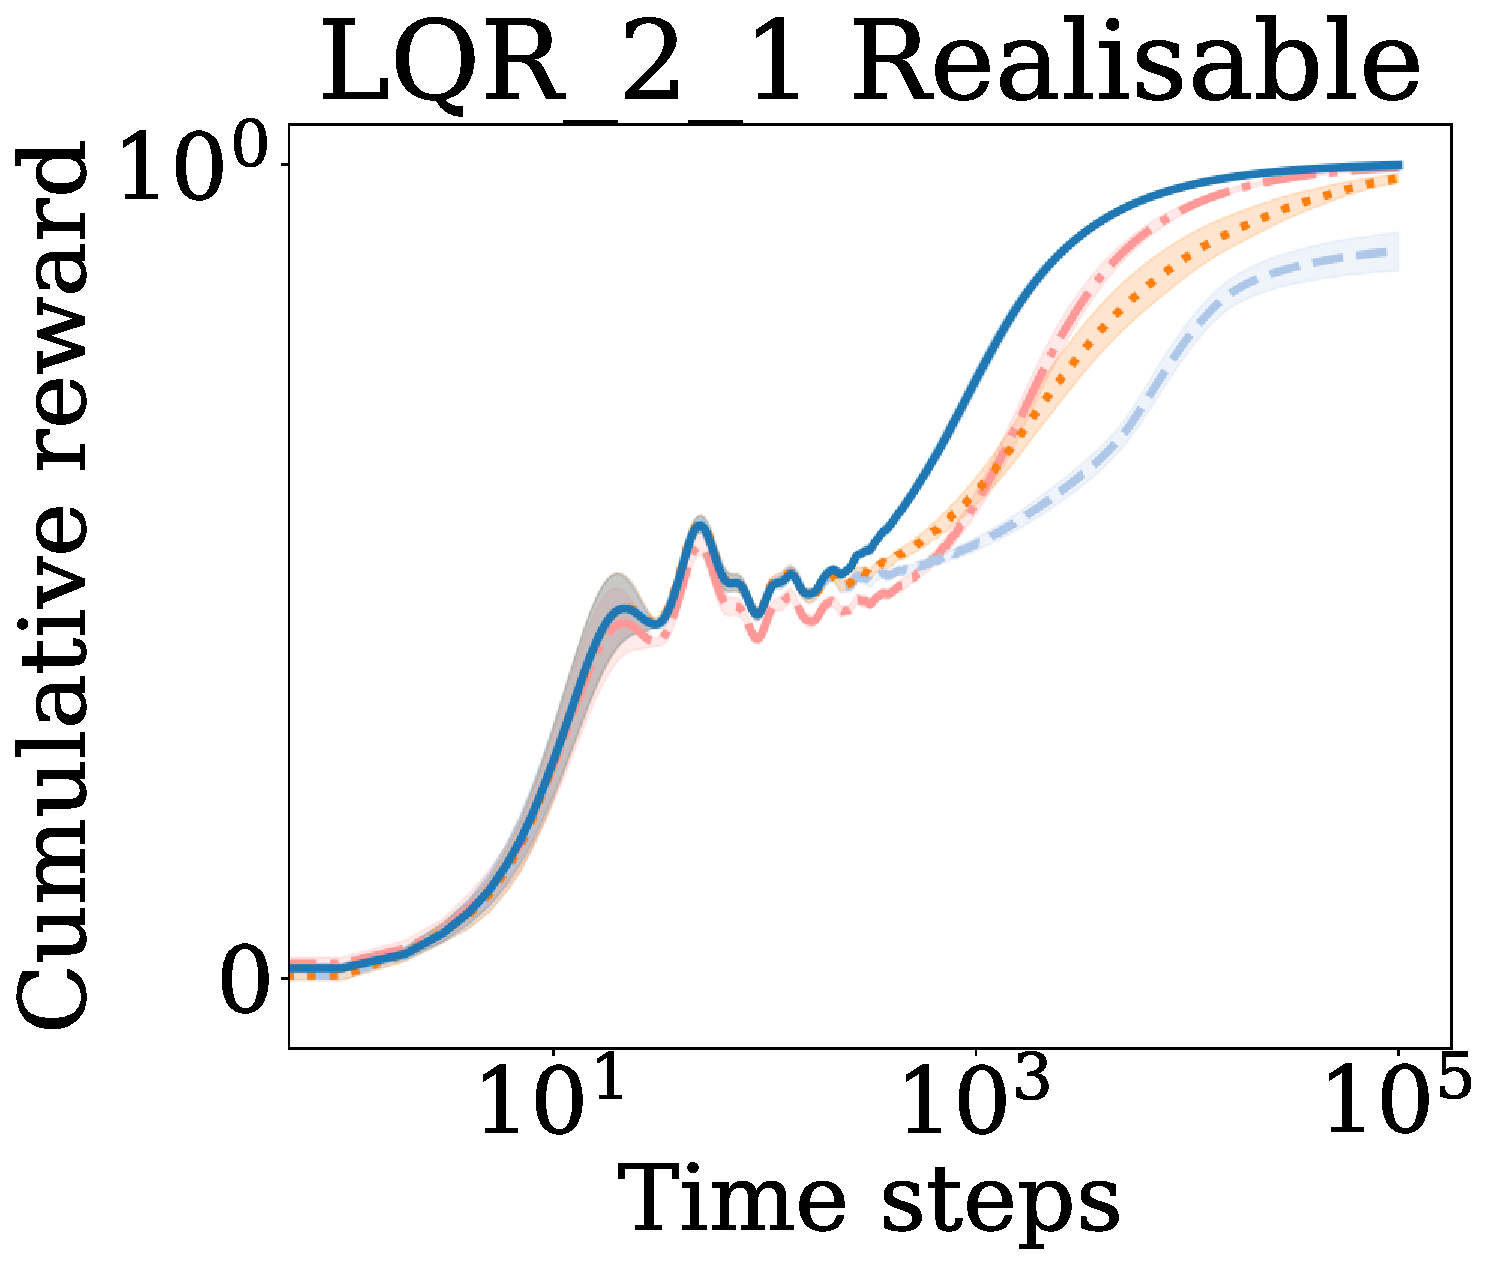
\includegraphics[width=0.3\textwidth]{img/lqr_2_1_realisable.pdf} 
    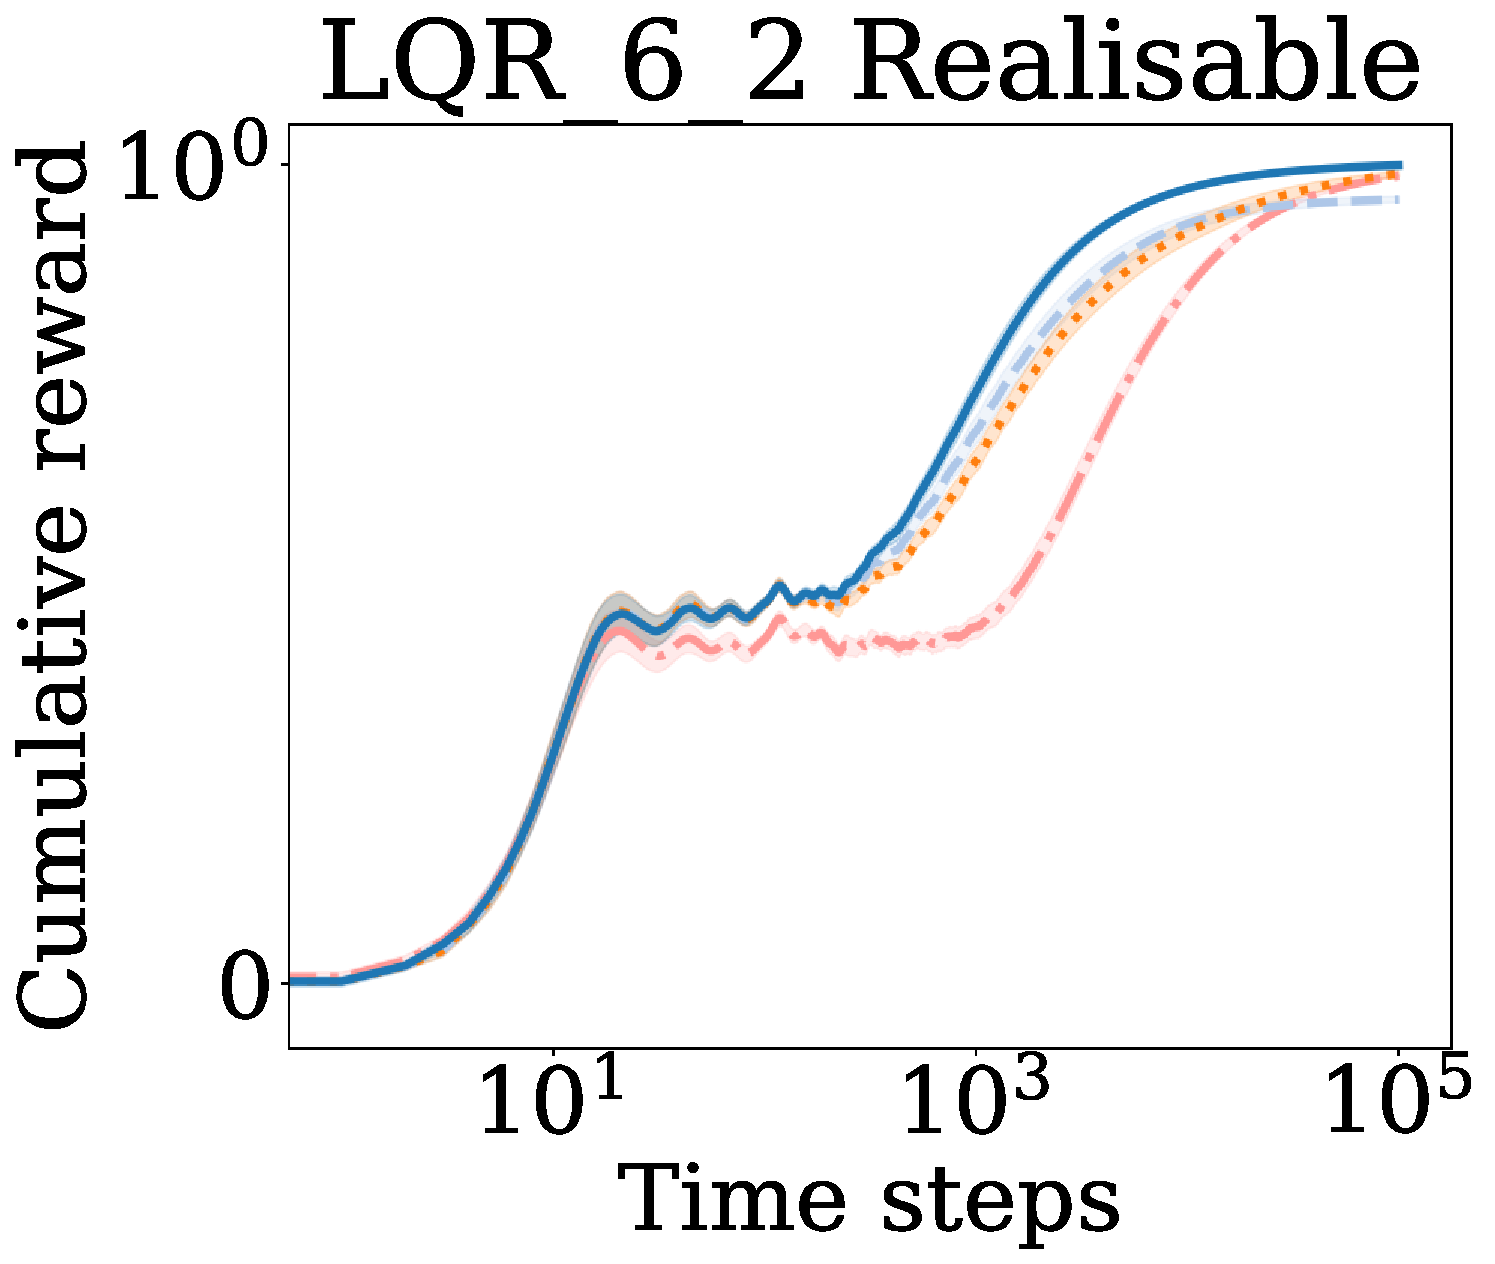
\includegraphics[width=0.3\textwidth]{img/lqr_6_2_realisable.pdf}\\
    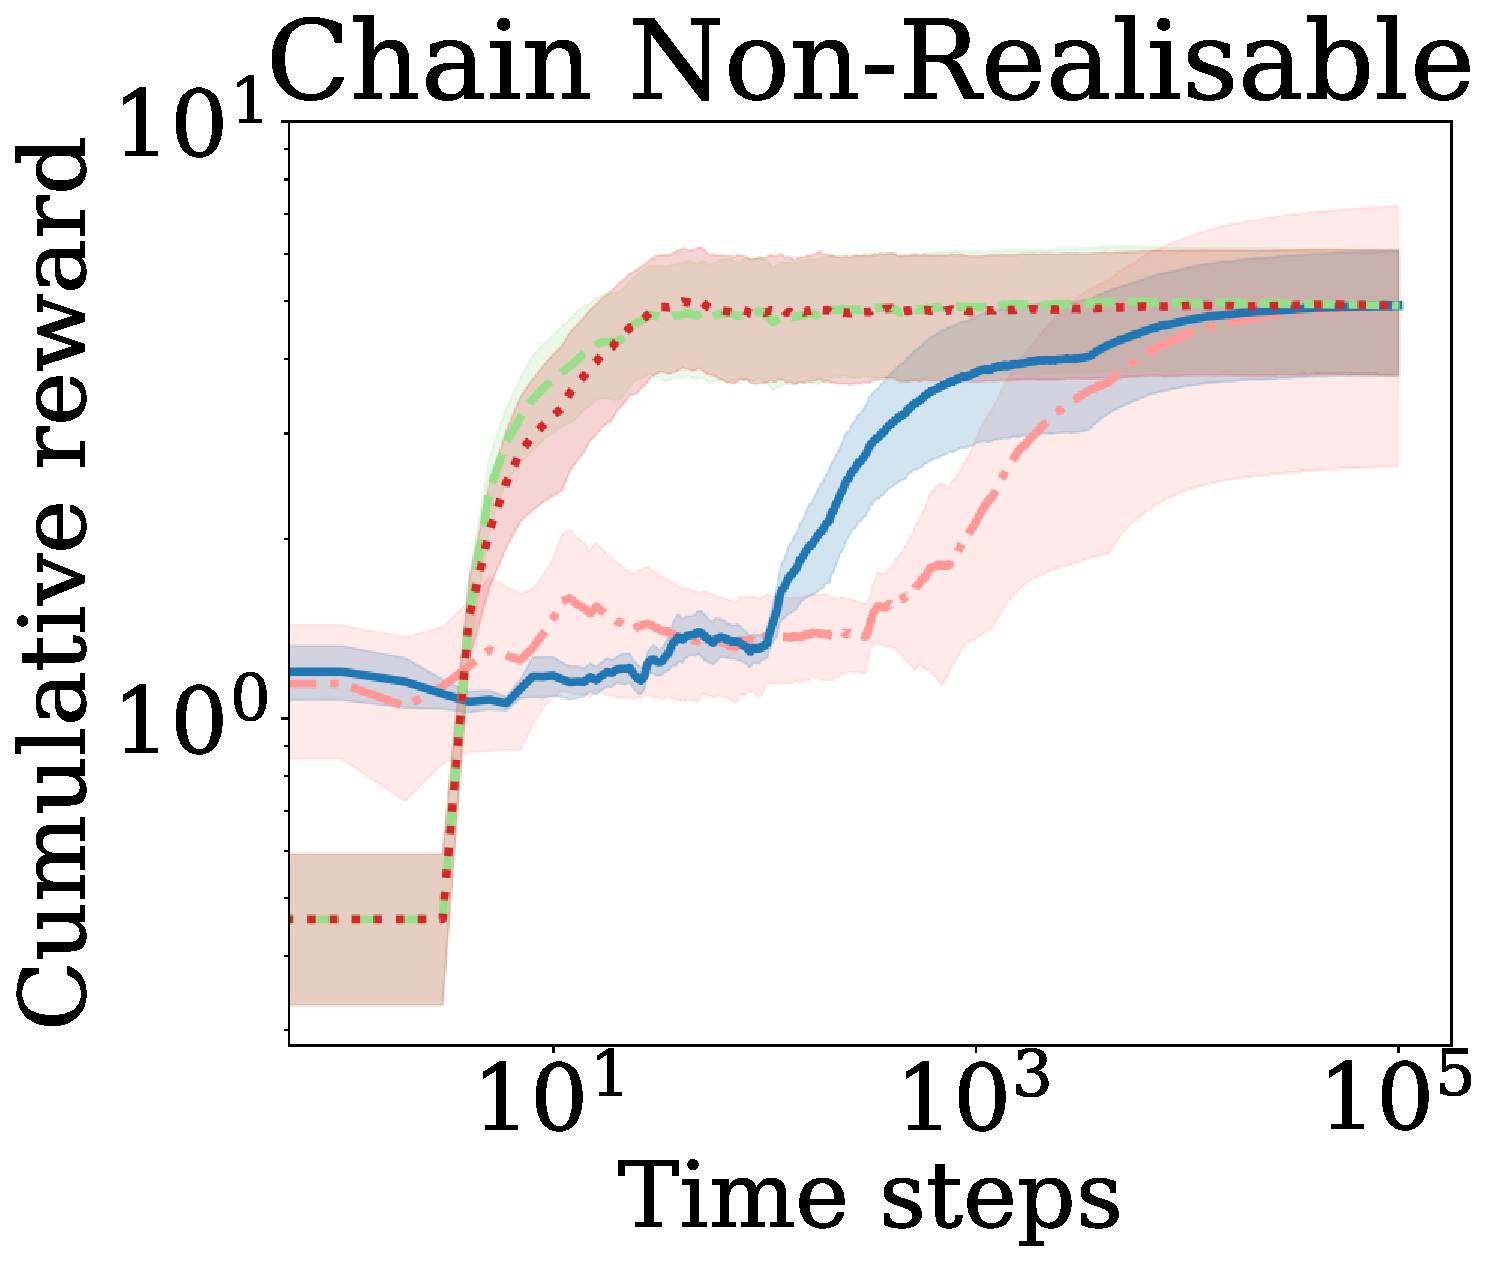
\includegraphics[width=0.3\textwidth]{img/chain_non_realisable.pdf}        
    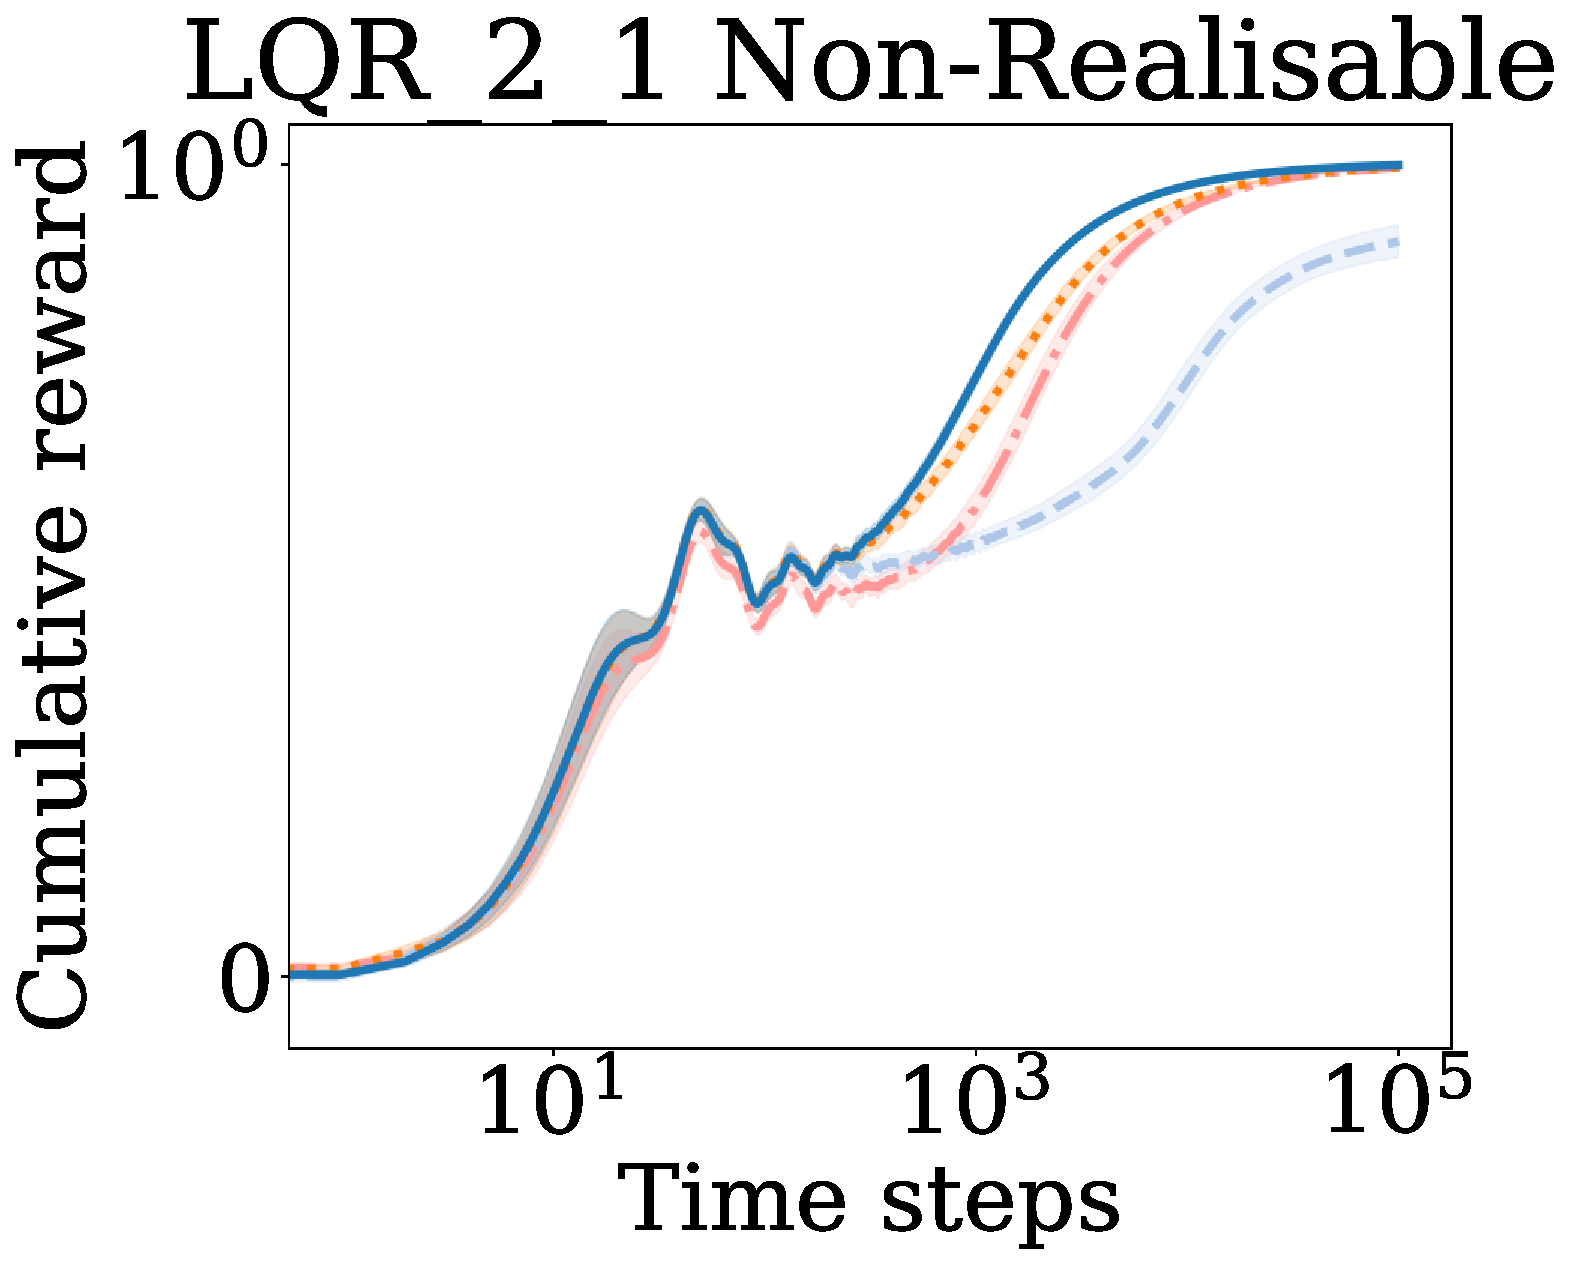
\includegraphics[width=0.3\textwidth]{img/lqr_2_1_non_realisable.pdf} 
    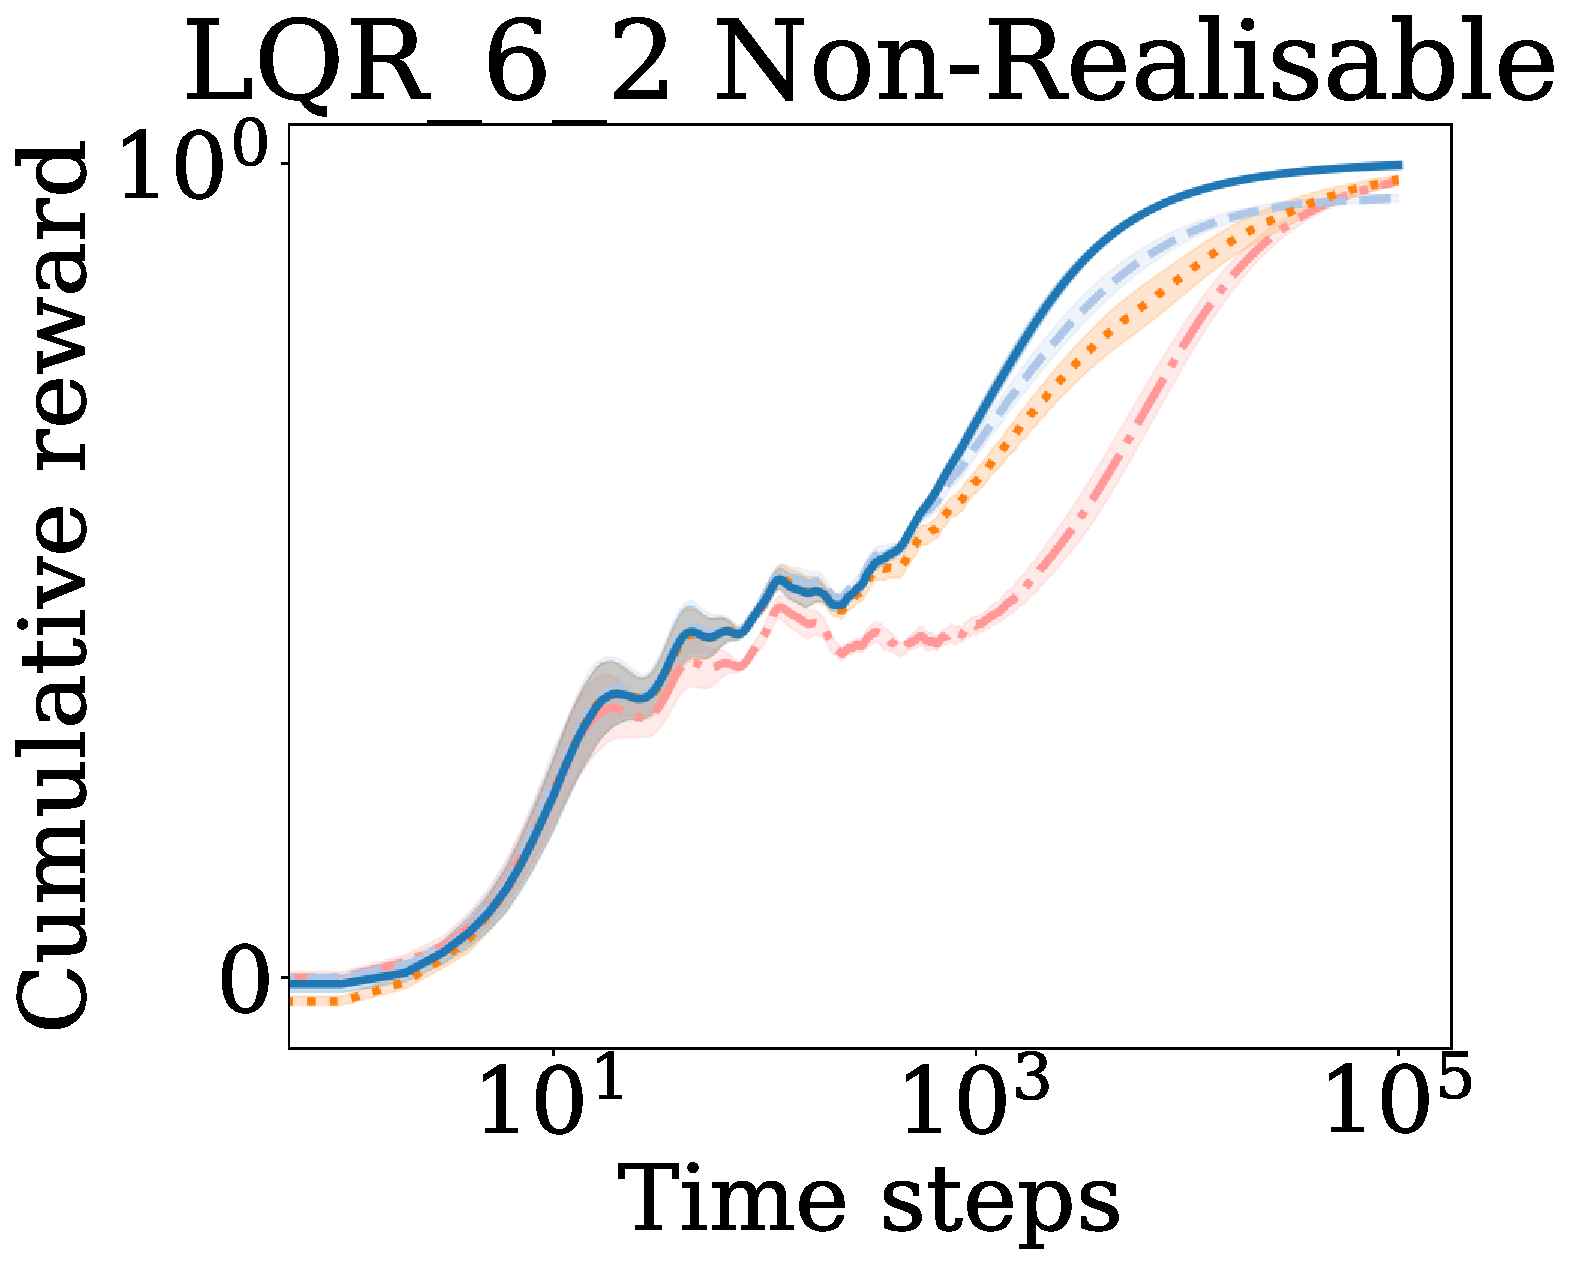
\includegraphics[width=0.3\textwidth]{img/lqr_6_2_non_realisable.pdf}\\
    
\includegraphics[width=0.9\textwidth]{img/lqr_legend.pdf}
    \caption{Depicted is the average cumulative reward at every time step computed over $10$ novel tasks in the realisable/non-realisable setting. The shaded regions represent the standard error of the average cumulative reward at the time step.}\label{fig:full_results}%\vspace*{-1em}
\end{figure}


\noindent\textbf{RL Environments.} We test the algorithms in a tabular MDP, i.e. Chain~\citep{dearden1998bayesian}, CartPole~\citep{barto1983neuronlike}, and two LQR tasks in \emph{Deepmind Control Suite}~\citep{tassa2018deepmind}: \\ \emph{dm\_LQR\_2\_1} and \emph{dm\_LQR\_6\_2}. %Further details on experimental setups are deferred to Appendix~\ref{sec:rl_env}.
Further details on experimental setups are deferred to Appendix C.1.


\noindent\textbf{(1) Impacts of Model Transfer with MLEMTRL.}\label{sec:impacts} We begin by evaluating the proposed algorithm in the Chain environment. The results of the said experiment are available in the leftmost column of Figure~\ref{fig:full_results}. In it, we evaluate the performance of MLEMTRL against PSRL, MT-PPO, MT-PPO-TRL. The experiments are done by varying the slippage parameter $p \in [0.00, 0.50]$ and the results are computed for each different setup of Chain from scratch. In this experiment, we can see the baseline algorithms MT-PPO and MT-PPO-TRL perform very well. This could partially be explained by PSRL and MLEMTRL not only having to learn the transition distribution but also the reward function. The value function transfer in the PPO-based baselines implicitly transfers not only the empirical transition model but also the reward function. We can see that MLEMTRL has improved learning speed compared to PSRL in both realisable and non-realisable settings. 
An additional experiment with a known reward function across tasks is shown in %Figure~\ref{fig:known_reward_results}. 
Figure 7 in Appendix.
%An additional experiment with known reward function across tasks is shown in Figure~\ref{fig:known_reward_results}. 

In the centre and rightmost columns of Figure~\ref{fig:full_results}, we can see the results of running the algorithms in the LQR settings with the baseline algorithms PSRL, MT-SAC and MT-SAC-TRL. The variation over tasks is given by the randomness over the stiffness of the joints in the problem. In these experiments, we can see a clear advantage of MLEMTRL compared to all baselines in terms of learning speed improvements, and in some cases, asymptotic performance.

In Figure~\ref{fig:full_results}, the performance metric is the average cumulative reward at every time step, for $10^5$ time steps and the shaded region represents the standard deviation, where the statistics are computed over $10$ independent tasks. %\\

%The average cumulative reward  and the shaded regions represent the $95\%$ confidence of the cumulative regret at the time step. The confidence interval is taken over the various variations of the Chain environment. The image clearly shows MLEMTRL has a jumpstart improvement coming as a result of the transfer learning scheme but also an indication of a learning speed improvement. 

\noindent\textbf{(2) Impact of Realisability Gap on Regret.} Now, we further illustrate the observed relation between model dissimilarity and degradation in performance. Figure~\ref{fig:norms} depicts the regret against the KL-divergence of the target model to the best proxy model in the convex set. We observe that model dissimilarity influences the performance gap in MLEMTRL. This is also justified in Section~\ref{sec:bounds} where the bounds have an explicit dependency on the model difference. In this figure, only the non-zero regret experiments are shown. This is to have an idea of which models result in poor performance. As its shown, it is those models that are very dissimilar. Additional results in %Figure~\ref{fig:time} further illustrate the dependency on model similarity.%\\
% Figure 5 in Appendix further illustrate the dependency on model similarity.


\begin{figure}[h]
    \centering
    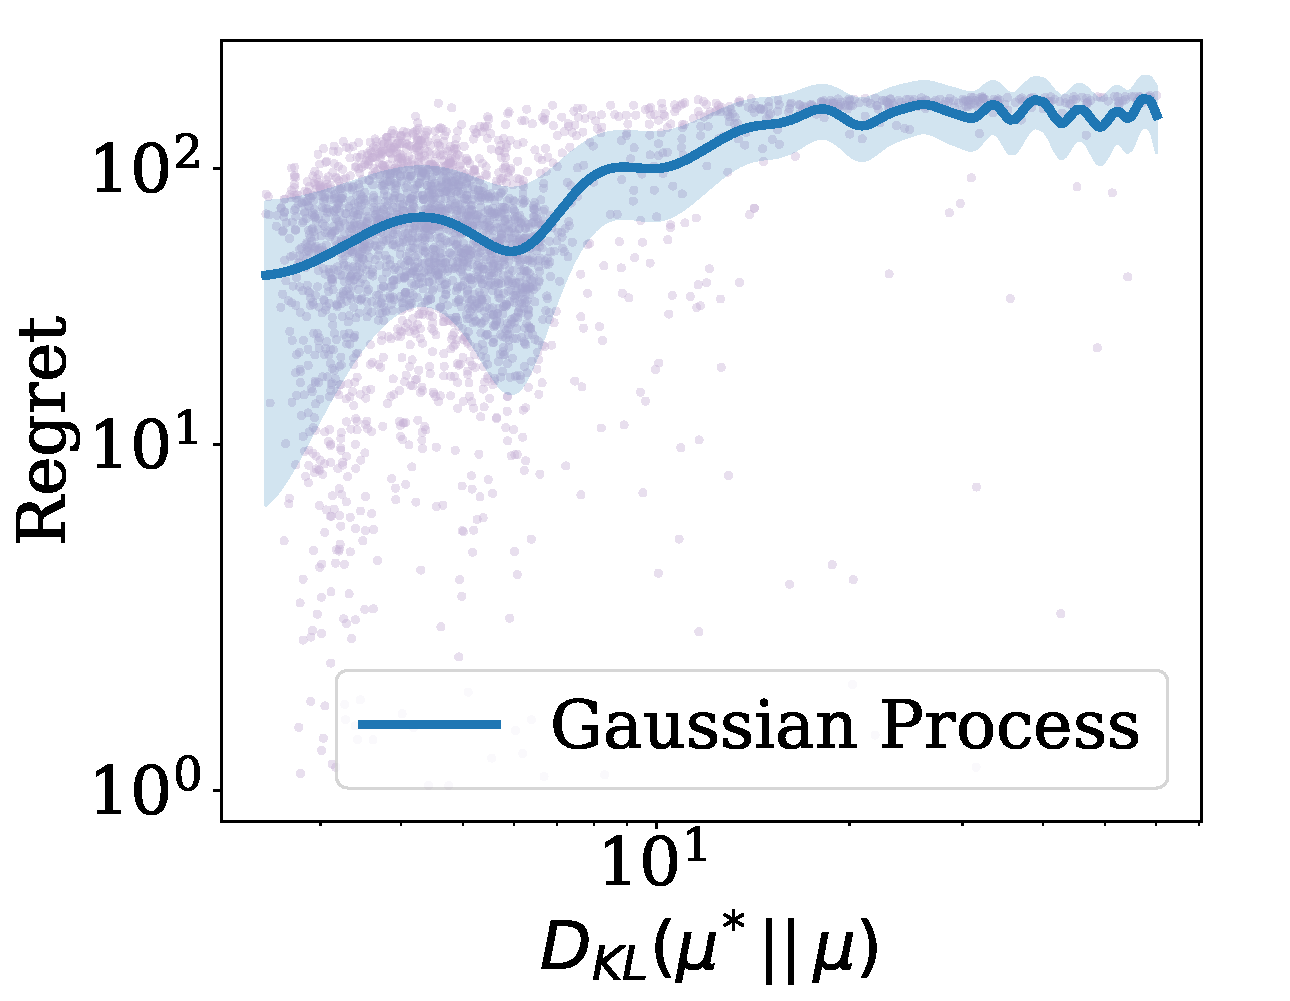
\includegraphics[width=.5\textwidth]{img/alpha_norms}
    \caption{A log-log plot of regret vs. KL-divergence between the true MDP and the best proxy model in CartPole. The thick blue line is a Gaussian Process regression model fitted on observed data (in purple).}
    \label{fig:norms}
\end{figure}

\begin{figure}[h]
    
    \centering
    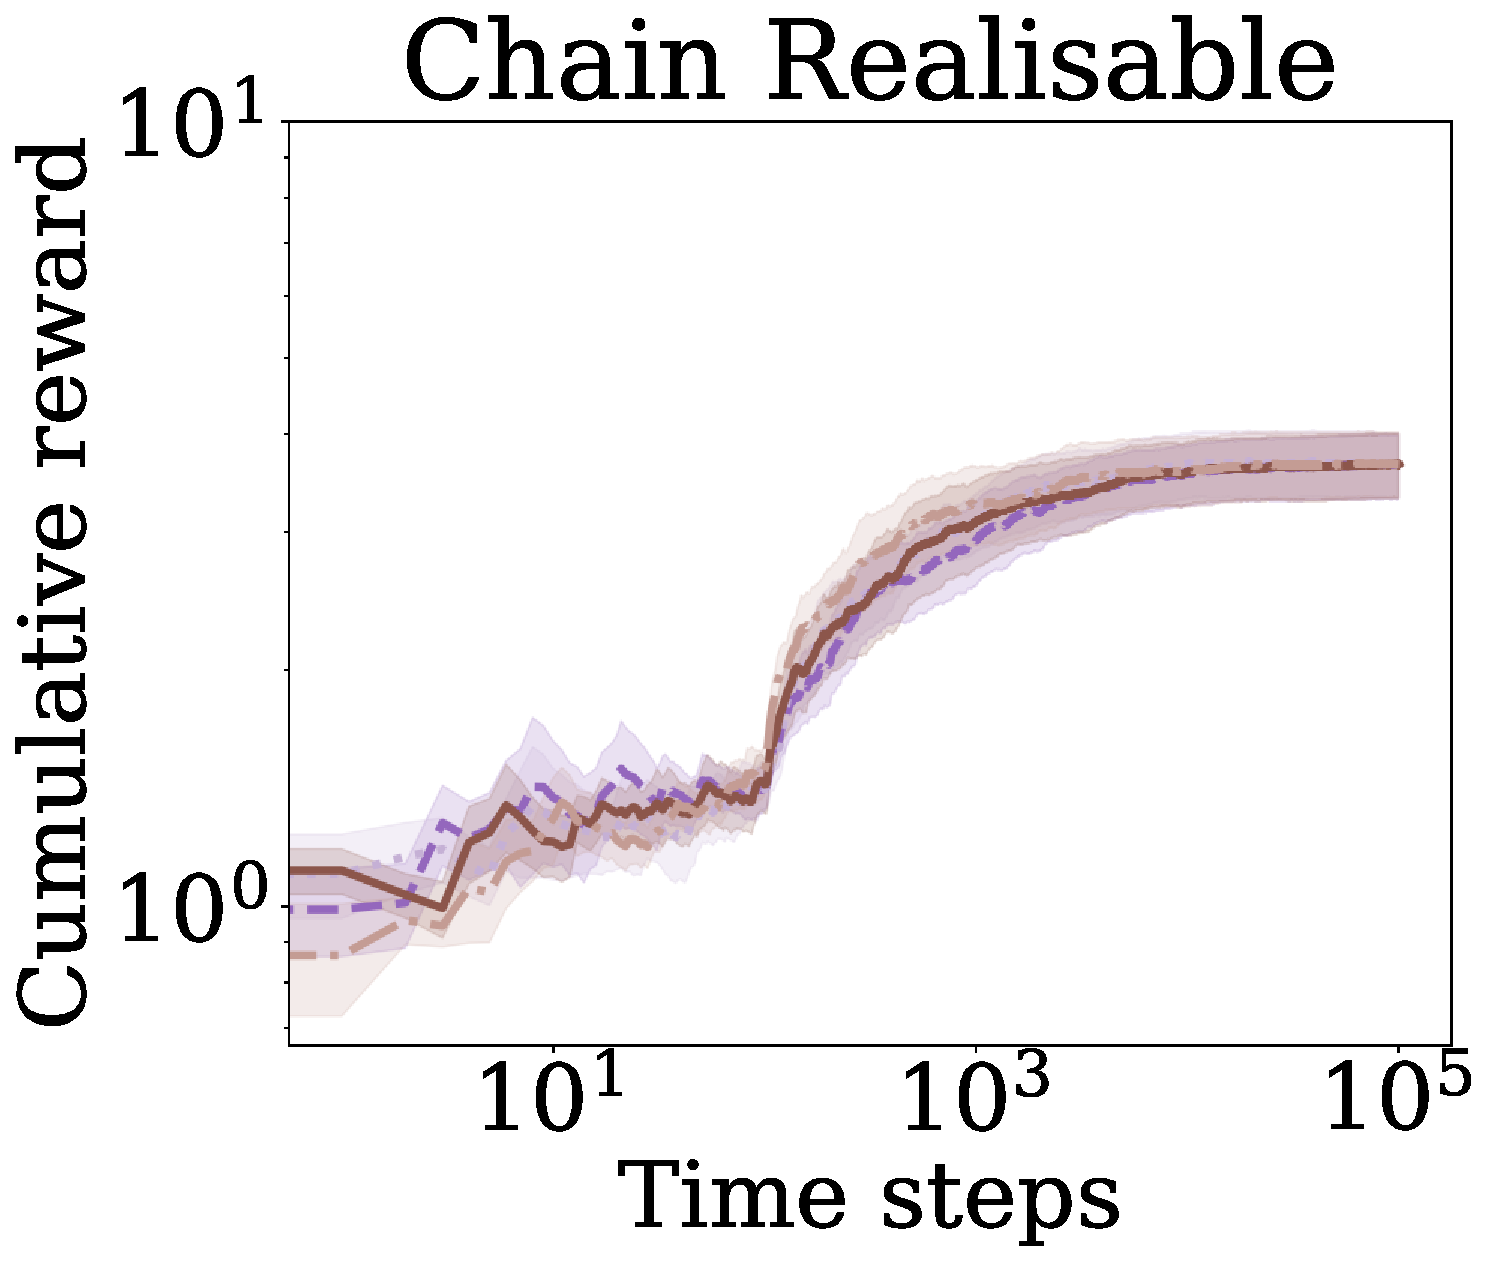
\includegraphics[width=0.48\textwidth]{img/chain_meta_realisable.pdf} 
    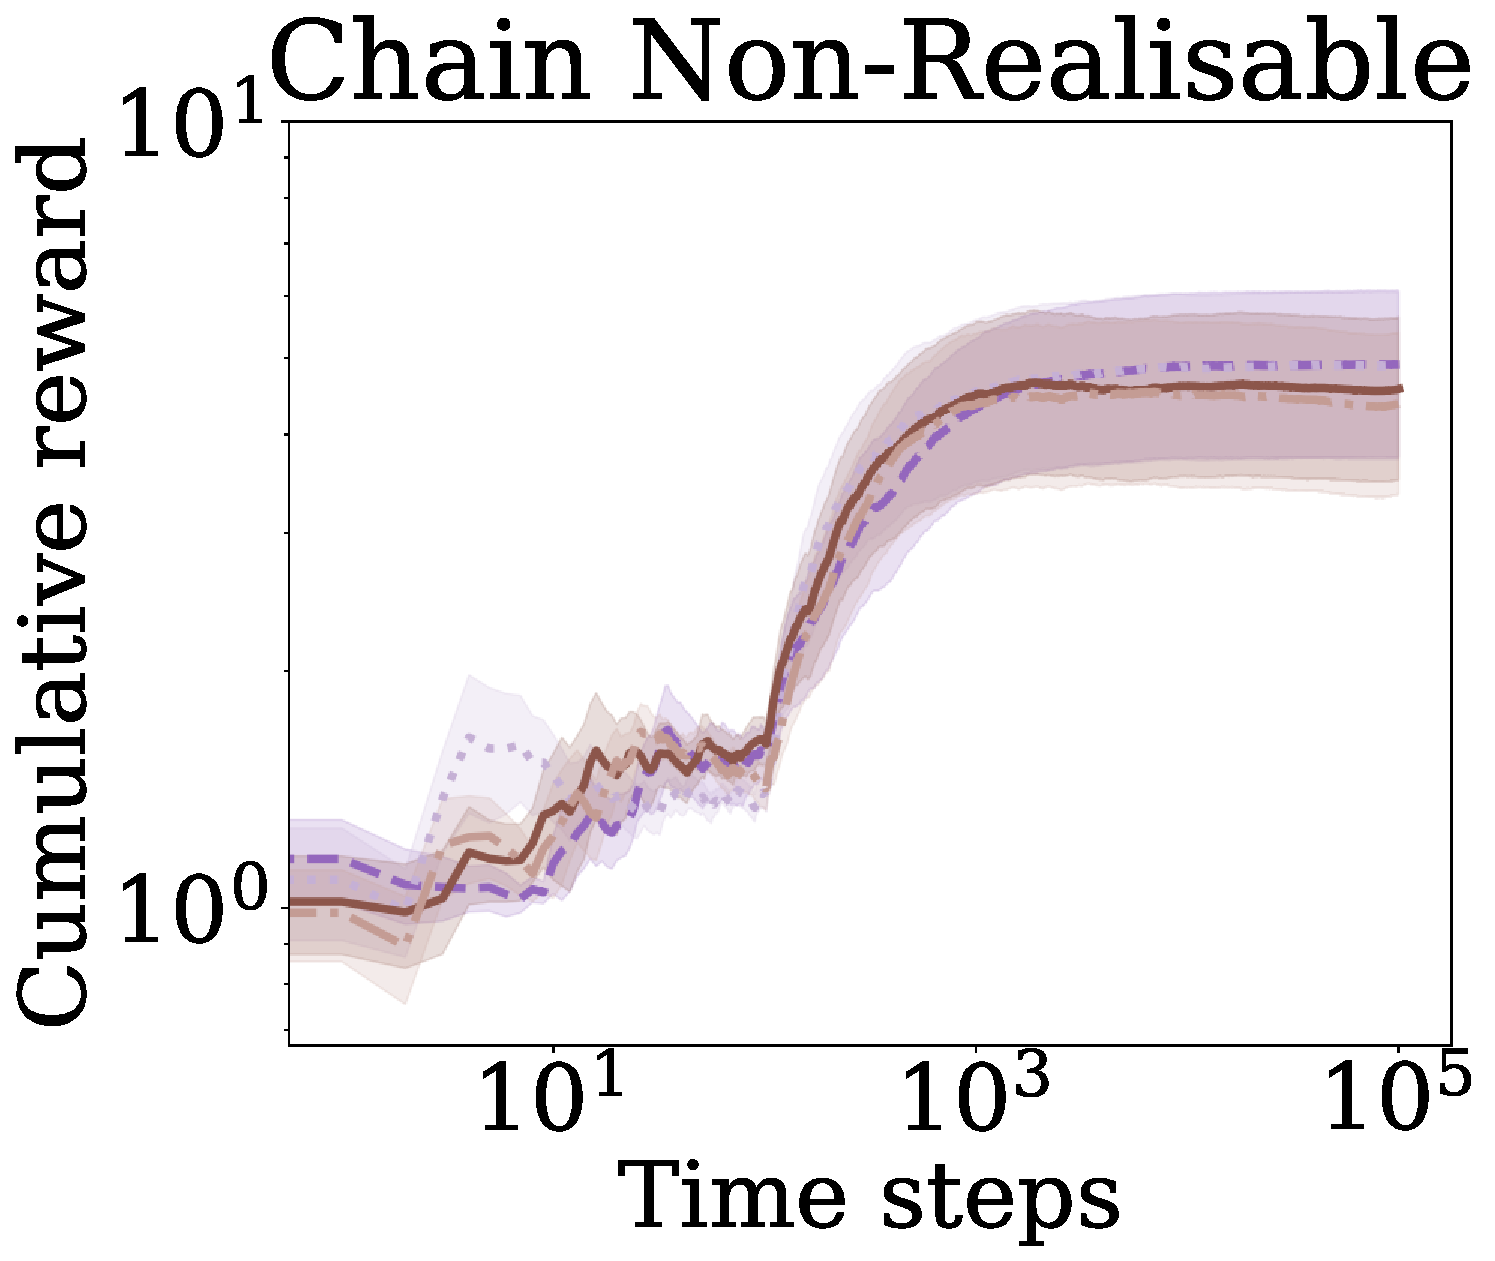
\includegraphics[width=0.48\textwidth]{img/chain_meta_non_realisable.pdf}\\
    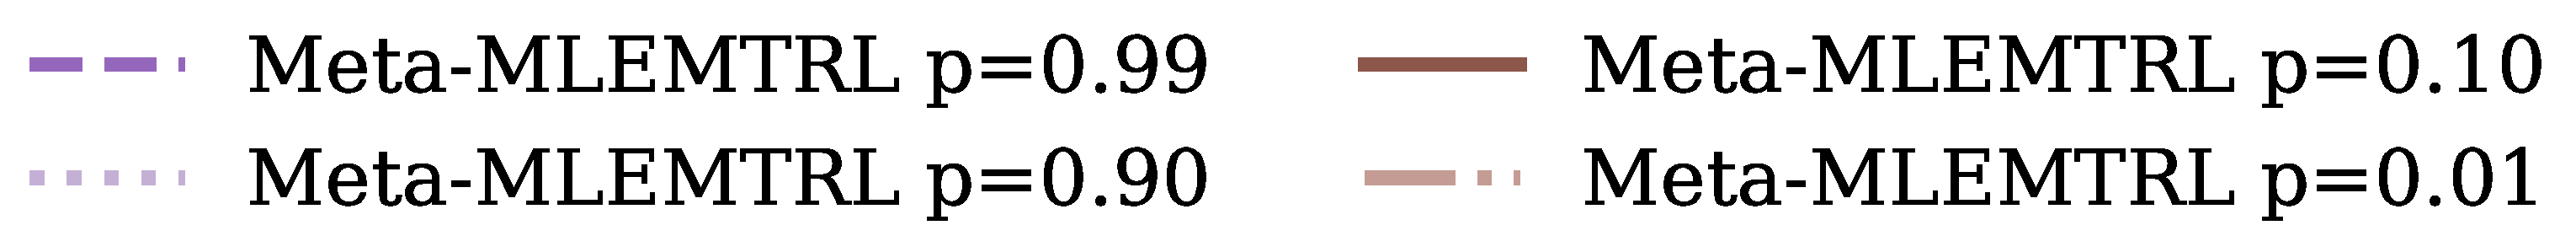
\includegraphics[width=0.9\textwidth]{img/lqr_legend3.pdf}
    \caption{Figure depicting an ablation study of the prior parameter $p$ in the Meta-MLEMTRL algorithm. The y-axis is the average cumulative reward at each time step computed over $10$ novel tasks and the shaded region represents the standard error. When $p=1$, the algorithm reduces to MLEMTRL and when $p=0$ the algorithm reduces to standard maximum likelihood model estimation.}
    \label{fig:meta_results}
\end{figure}


% \begin{figure*}[t!]
% \centering
%     \begin{minipage}{0.34\textwidth}
%     \centering
%     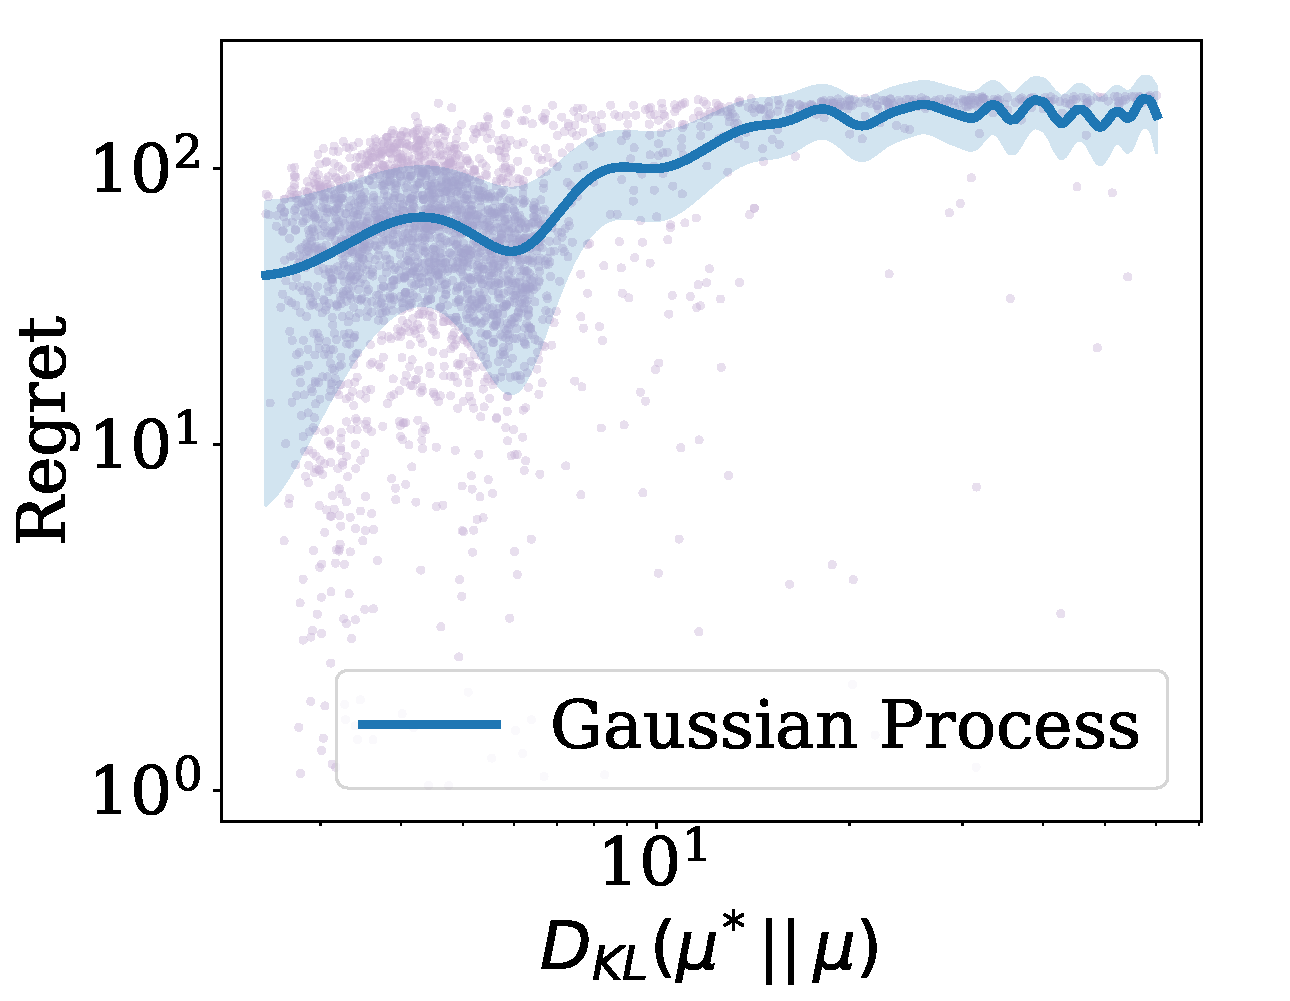
\includegraphics[width=\textwidth]{img/alpha_norms}\\~\\~\\
%     \caption{A log-log plot of regret vs. KL-divergence between the true MDP and the best proxy model in CartPole. The thick blue line is a Gaussian Process regression model fitted on observed data (in purple).}\label{fig:norms}%Only the non-zero regret results are displayed to indicate how sub-optimal performance relates to model dissimilarity. 
%     \end{minipage}\hfill
%     \begin{minipage}{0.65\textwidth}
%     \centering
%     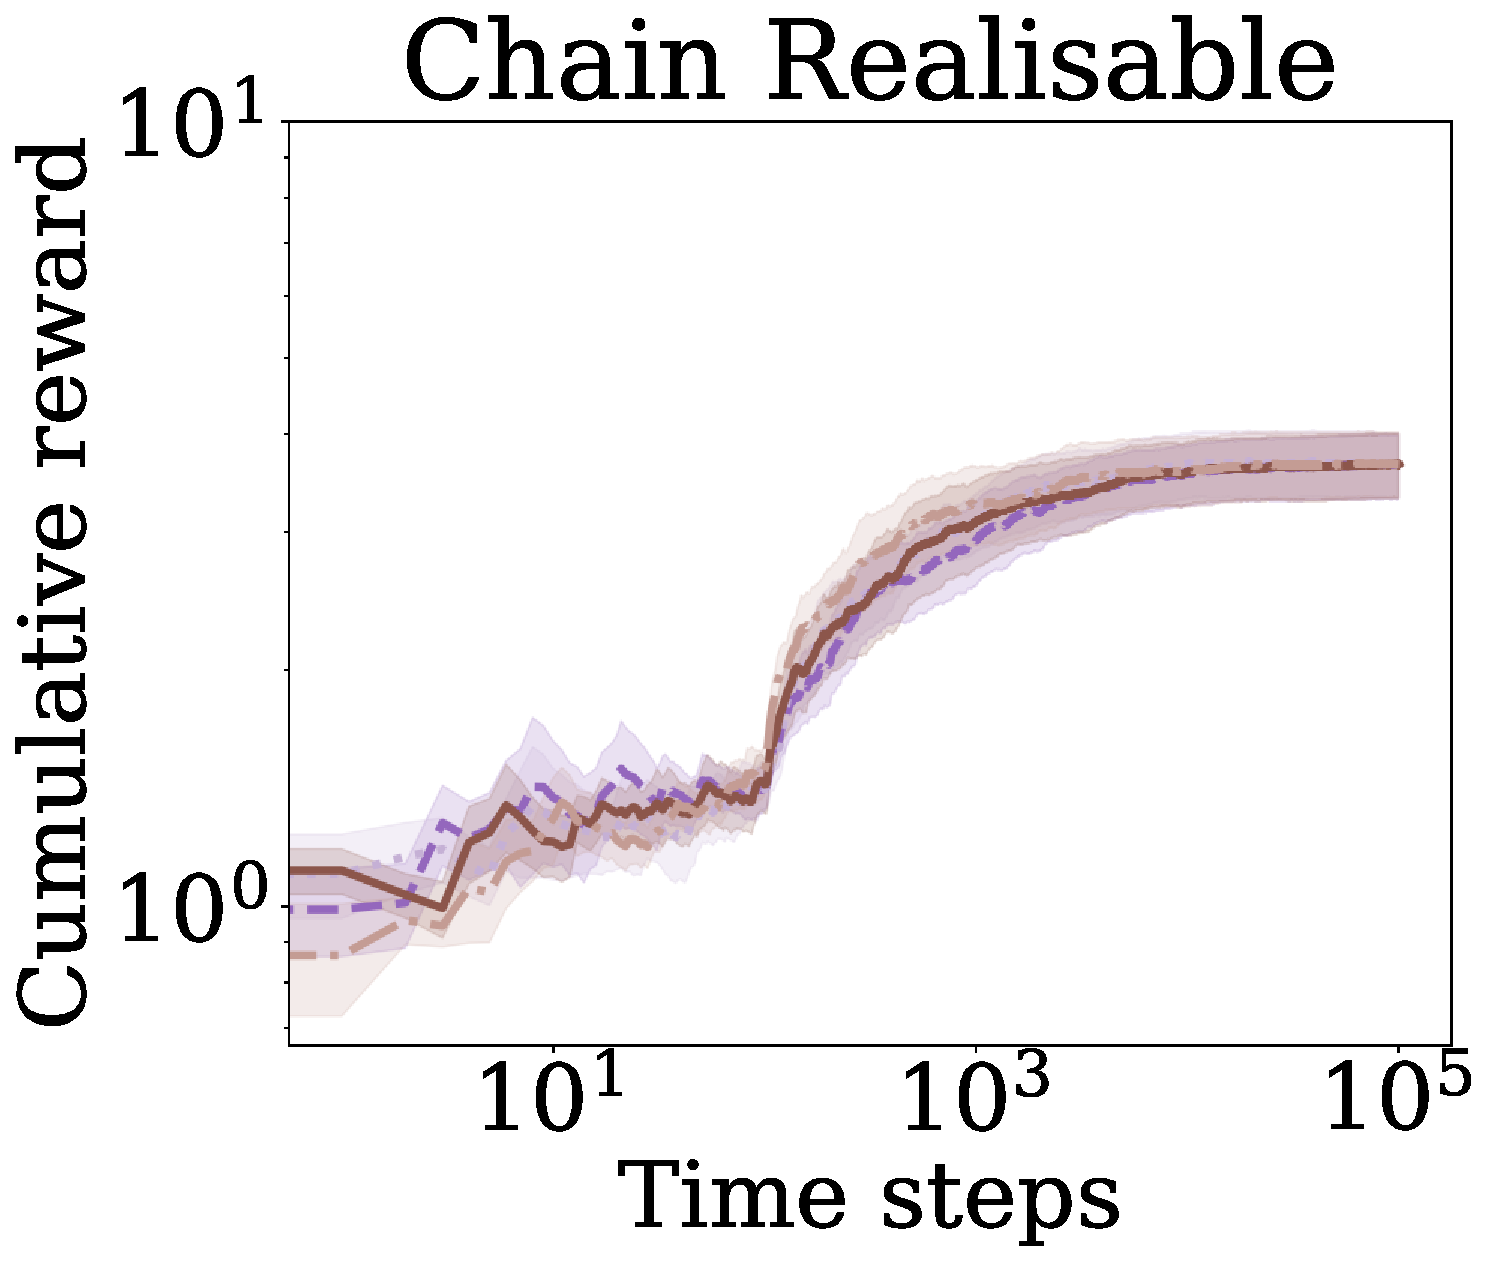
\includegraphics[width=0.48\textwidth]{img/chain_meta_realisable.pdf} 
%     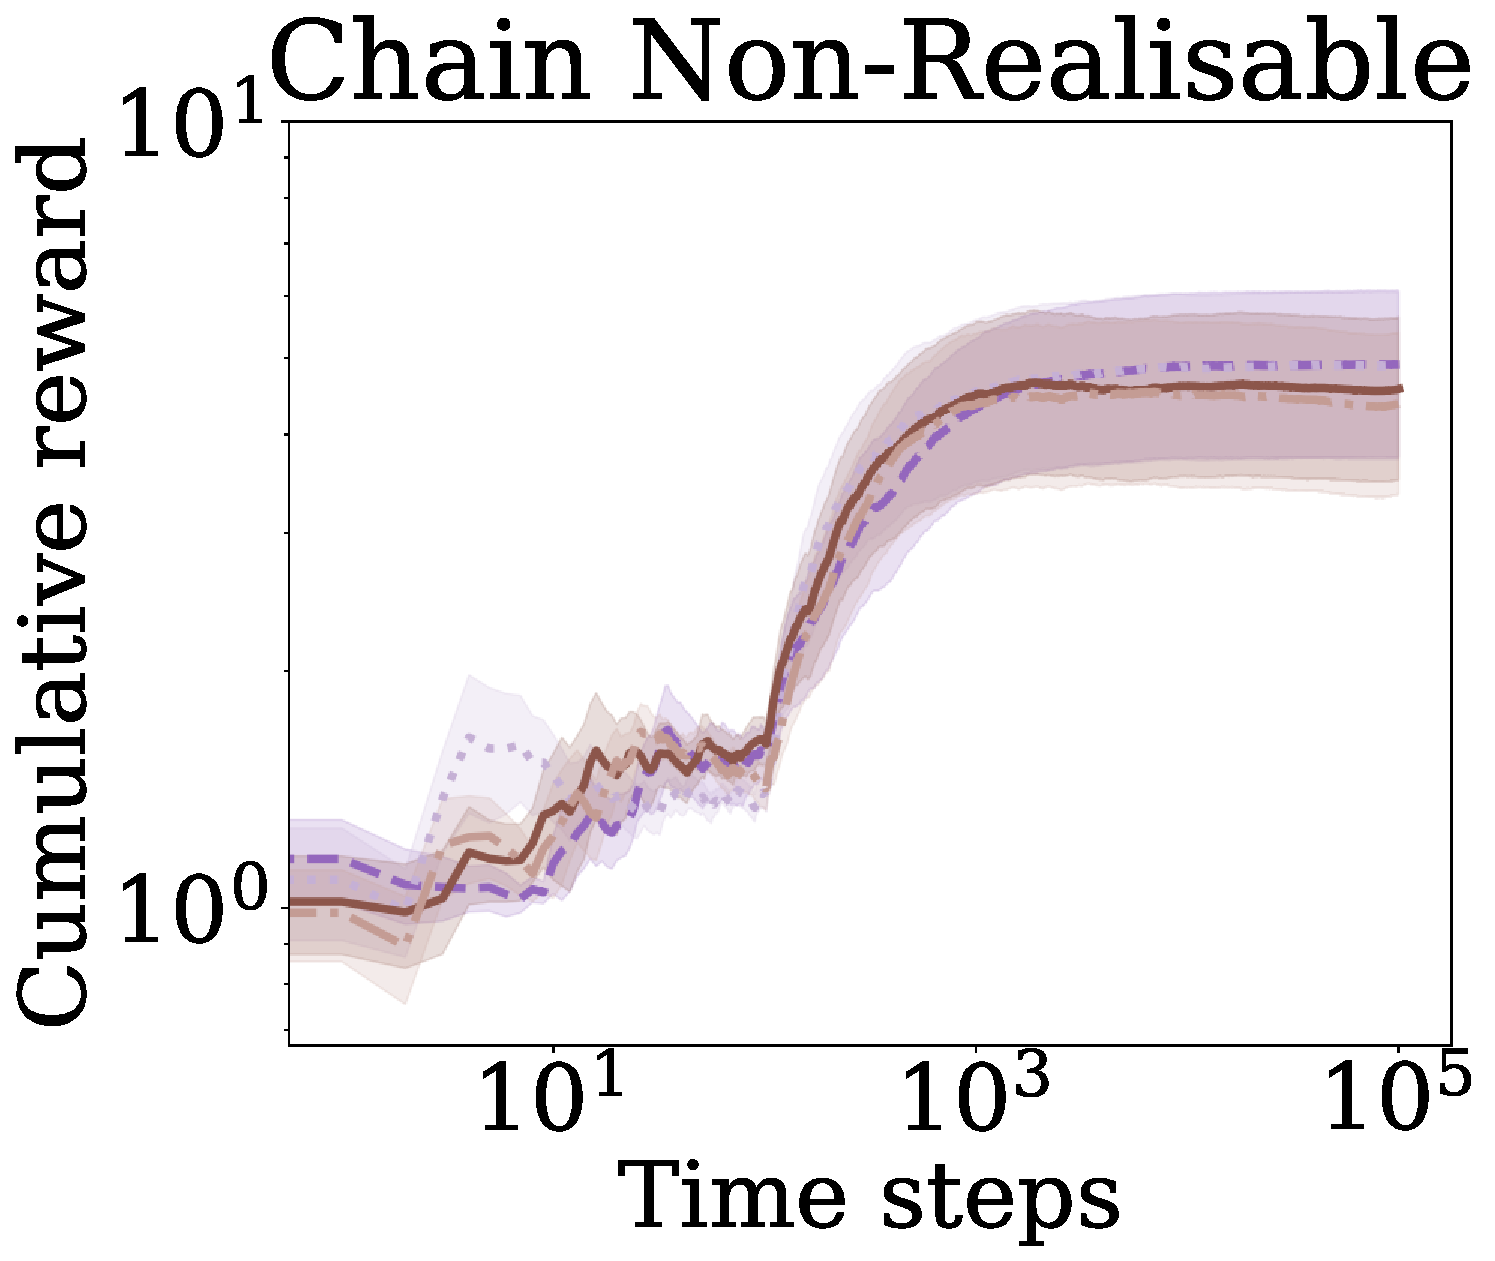
\includegraphics[width=0.48\textwidth]{img/chain_meta_non_realisable.pdf}\\
%     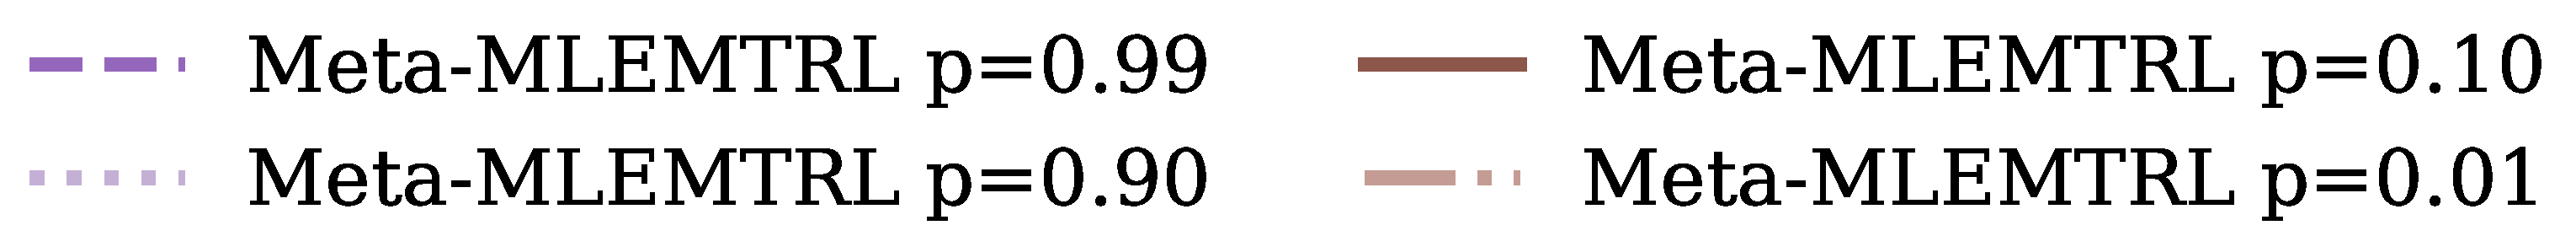
\includegraphics[width=0.9\textwidth]{img/lqr_legend3.pdf}
%     \caption{Figure depicting an ablation study of the prior parameter $p$ in the Meta-MLEMTRL algorithm. The y-axis is the average cumulative reward at each time step computed over $10$ novel tasks and the shaded region represents the standard error. When $p=1$, the algorithm reduces to MLEMTRL and when $p=0$ the algorithm reduces to standard maximum likelihood model estimation.}\label{fig:meta_results}
%     \end{minipage}
% \end{figure*}

\noindent\textbf{(3) Performance of Meta-MLEMTRL under Non-realisability.} In order to validate the performance of the proposed meta algorithm Meta-MLEMTRL, we perform an ablation study over the prior hyperparameter $p$. In Figure~\ref{fig:meta_results}, we illustrate the results of running the Meta-MLEMTRL algorithm in the Chain environment for both the realisable and non-realisable settings. The choice of $p$ determines how much the algorithm should be biased towards the model estimated using MLEMTRL and in the case when $p=1$, Meta-MLEMTRL reduces to MLEMTRL. Similarly, if $p=0$ then the algorithm will forego the MLEMTRL-estimate for the empirical estimate. Figure~\ref{fig:meta_results} shows that the performance of Meta-MLEMTRL is stable in long-run for different values of $p$. %More experiments would be needed in order to make any strong empirical claims, 
However, we identify that higher $p$ values yield positive improvements in the cumulative reward over $10^5$ steps, especially in the non-realisable setting. This indicates that the MLEMTRL-estimated model acts a good representation, while combined with the asymptotically converging empirical estimate obtained by Meta-MLEMTRL.%\\

\noindent\textbf{Summary of Results.} In the experiments, we sought to identify whether the proposed algorithm shows superiority in terms of the transfer learning goals given by~\citep{langley2006transfer}. In the LQR-based environments, we can see a clear superiority of MLEMTRL in terms of learning speed compared to all baselines and in some cases, an asymptotic improvement. In the Chain environment, the proposed algorithm, MLEMTRL, outperforms PSRL in terms of learning speed. Also, we perform an ablation study of Meta-MLEMTRL under realisable and non-realisable settings, demonstrating provable improvements in the asymptotic and non-realisable regimes.

%In our first experiment, we see a clear superiority in terms of learning speed and jumpstart improvement. These results are consistent for the second experiment as well, given that the true MDP is similar enough to the source tasks. In the second and third experiment we verify the claim that a loss in performance (in terms of regret) has a strong dependence on the dissimilarity of the estimated MDP and the true MDP.

%Additional ablative experiments showing how the performance loss increases with model dissimilarity is available in Figure~\ref{fig:norms}, how MLEMTRL can be augmented with an hierarchical procedure to take the empirical model into account in addition to the source models in Figure~\ref{fig:meta_results} and in Figure~\ref{fig:sac_results}, showing how the use of multi-task and transfer reinforcement learning may improve the performance over a standard RL approach.

%Additional ablation studies showing how MLEMTRL can be augmented with a hierarchical procedure to take the empirical model into account in addition to the source models are depicted in Figures~\ref{fig:meta_results} and~\ref{fig:sac_results}. They show how the use of multi-task and transfer RL can improve performance over a standard RL approach. 

%Additional ablative experiments showing how MLEMTRL can be augmented with an hierarchical procedure to take the empirical model into account in addition to the source models in Figure 4 and in Figure 5, showing how the use of multi-task and transfer reinforcement learning may improve the performance over a standard RL approach.

